\chapter{Schemi di rete}
\label{appendix:schemi}

\section{Slide Sangfor: posizionamento consigliato delle sonde}
\label{network:sangfor-sta-position}

\begin{figure}[!htbp]
    \centering
    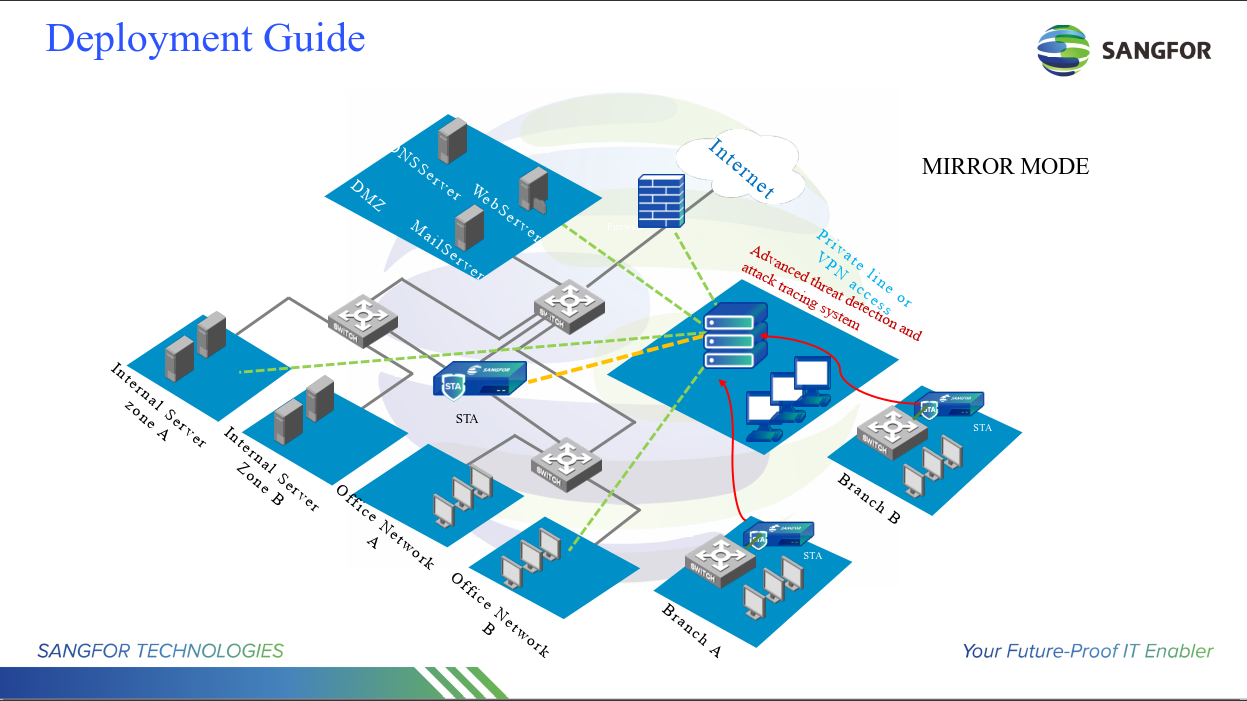
\includegraphics[width=0.8\linewidth]{images/ndr/sangfor-posizionamento.png}
    \caption{Configurazione di esempio del produttore}
    \label{fig:sangfor-sta-position}
\end{figure}

\pagebreak

\section{Rete Wintech: posizionamento delle sonde tra le sedi}
\label{network:wtc-sta-position}

\begin{figure}[!htbp]
    \centering
    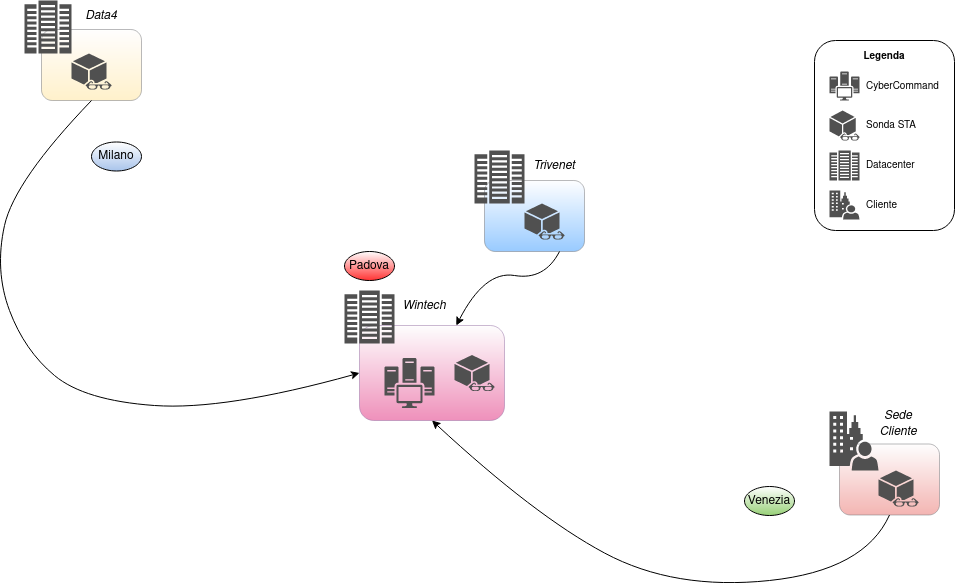
\includegraphics[width=\textwidth]{images/ndr/sonde.png}
    \caption{Posizionamento delle sonde}
    \label{fig:wtc-sta-position}
\end{figure}

\pagebreak

\section{Segnalazione richieste DNS malevole: schema qualitativo}
\label{network:dns-multiple-request}

\begin{figure}[!htbp]
    \centering
    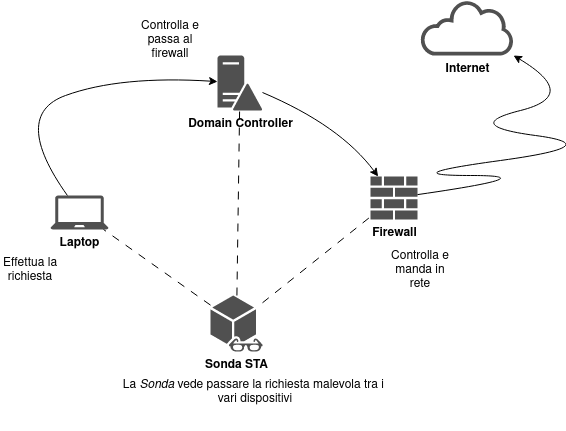
\includegraphics[width=1\linewidth]{images/ndr/dns-req.png}
    \caption{Richieste DNS rilevate dal sistema}
    \label{fig:cc-dns-req}
\end{figure}
